Meetings with multiple speakers can be challenging for individuals who require accessibility accommodations, such as hard-of-hearing people. Audio-to-text conversion has been a helpful tool to assist these individuals. Still, it does not address the issue of identifying the speaker in a meeting and generating a summary for the given meeting. Therefore, there is a need for a pipeline that can identify the speaker and summarize a given audio file. Besides granting accessibility accommodations to hard-of-hearing people, we also want to provide accurate and insightful analysis to customers and researchers, which can help them understand and utilize the content of the meetings better. In addition to providing accessibility accommodations for individuals who are hard of hearing, we want to offer precise and insightful analysis to both customers and researchers. This analysis can improve their comprehension and utilization of meeting content. This can be especially beneficial for organizations that need to monitor multiple meetings and extract key information for decision-making and research purposes.



\begin{figure*}[thbp]
	\centering
	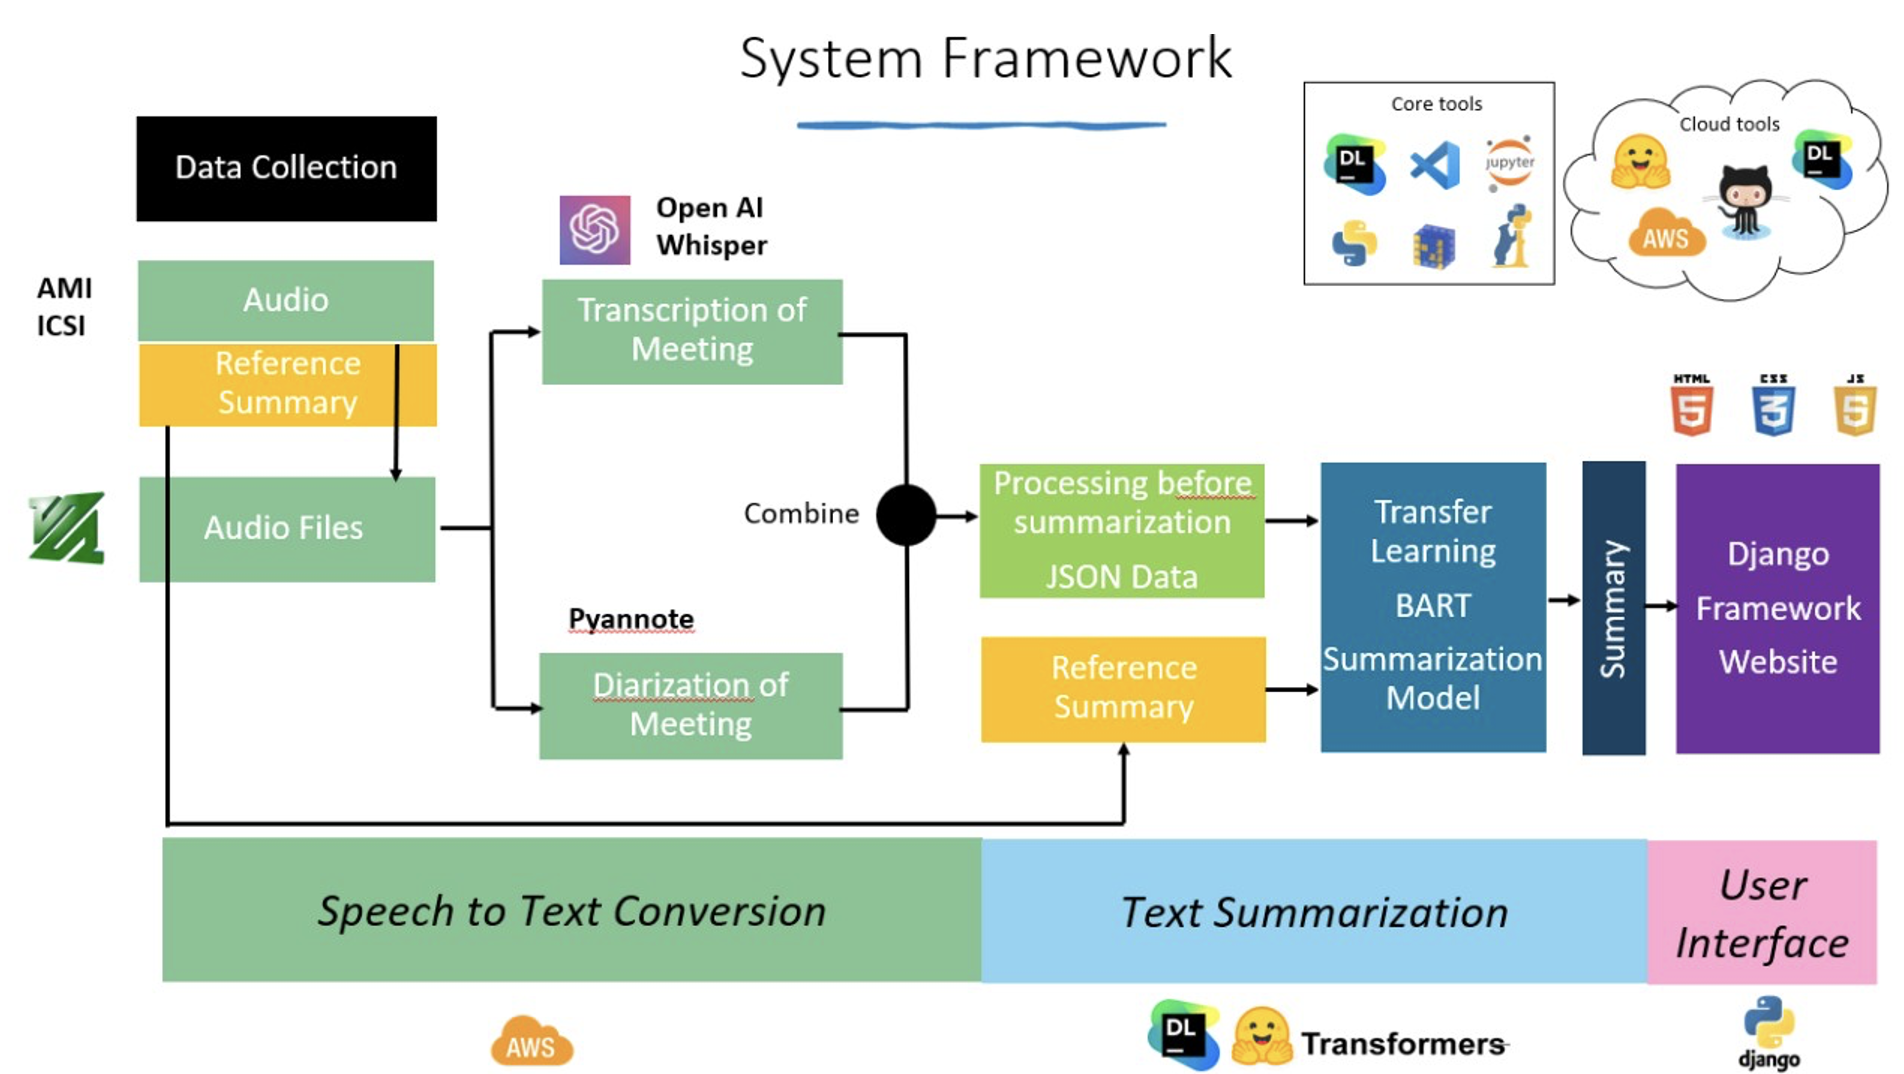
\includegraphics[width=14cm, height=6cm]{figures/overview}
	\caption{An overview of system framework}
	%\Description{Overview}
	\label{fig:overview}
	\textcolor{red}{will need to replace with a new figure. remove title and tool figures. reduce \# colors and bigger/clearer font}
\end{figure*}




We aim to conduct audio analysis from speech to text specifically in conversations with more than two speakers in a meeting environment. Besides granting accessibility accommodations to hard-of-hearing people, we also want to provide an accurate and insightful analysis for customers and researchers to leverage.

This audio analysis problem can be partitioned into four different parts:

\begin{itemize}
\item Automatic Transcription: We used OpenAI’s Whisper to automatically transcribe audio files.

\item Speaker Diarization: We used an opensource Python library called Pyannote to perform basic speaker diarization.

\item Summarization: We used a pre trained BART model trained on the CNN/Dailymail and SAMSUM datasets.

\item Visualization/Presentation: We developed a basic front-end web application where users can upload an audio file and receive a transcript and summary.

\end{itemize}

We created a working summarization pipeline starting with an Automatic Speaker Recognition (ASR) module consisting of OpenAI Whisper and Pyannote. For our summarization module, we performed transfer-learning on a pre trained BART sequence-to-sequence transformer model by training the model on a machine transcribed AMI/ICSI corpus to improve summarization for long meetings.

